\chapter{Introduction}
The implemented high-level synchronization component in this master thesis is part of the KIA4SM project of the department of operating systems. The work aims to implement a method for dynamic update of tasks ready queues in L4 Fiasco.OC/Genode while providing a synchronized access to them.



  

\section{Overview of KIA4SM project}

KIA4SM (stands for Cooperative Integration Architecture for Future Smart Mobility Solutions) is a research project at the department of operating systems. Traditionally Cooperative Intelligent Transport Systems have been built on heterogeneous systems. KIA4SM aims to provide an architecture of having an homogeneous platform for heterogeneous systems. 

KIA4SM focuses on developing systems for the interaction and coordination between
computer-assisted vehicles, be it partially or fully autonomously functioning actors.  KIA4SM aims to improve on the ad-hoc networking between vehicles

The final vision of the project is illustrate in figure \ref{kia4sm}. The goals of the project are,

\begin{figure}[kia4sm]
  \centering
  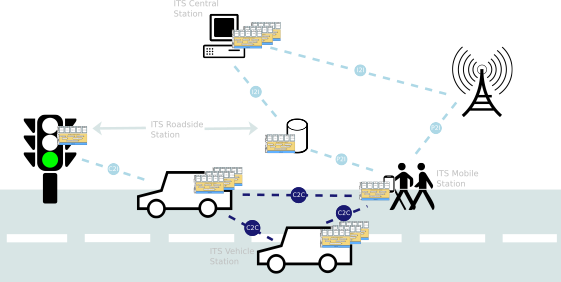
\includegraphics[scale = 1]{figures/kia4sm_vision.png}
  \caption{KIA4SM vision - homogeneous platform for heteroge-
  neous devices}\label{kia4sm}
\end{figure}

\begin{itemize}
\item A common platform as foundation for device in-
dependent (vehicles, mobile devices, traffic and
transport architecture) provision and execution of
software-based functionality
\item Mechanisms that allow for online dynamic reconfig-
uration, based on
\begin{itemize}
\item en-/disabling and relocation/migration of
software-based functionality
\item adaptive (data-centric) routing policy
\item flexible scheduling of tasks per ECU
\end{itemize}
\end{itemize}

In order to achieve the goals of the project a number of different methods have been applied. This has led to the application of Organic computing paradigm. igner and user.
Organic Computing (OC) has the vision to address the
challenges of complex distributed systems by making them more
life-like (organic), i.e. endowing them with abilities such as self-
organization, self-configuration, self-repair, or adaptation.
%Refer: paper: Organic Computing – Addressing Complexity by Controlled Self-organization 
In order to realize this, universally applicable Electronic Control Units (ECU) and a common run-time environment are used which provides Hardware/Software Plug-and-Play properties.

\section{Motivation}

There are number of micro controllers used for different calculations in a modern vehicle, this project aims to replace them with use more power-full and standardized hardware universally applicable ECUs. 

OC approach proposes a Observer-Controller architecture similar to MAPE architecture(monitor, analyze, plan, execute) . An observer collects the data from the all the ECUs and computes and generates indicators where a controller takes a decision based on the indicator, generates an action.

One such action of the controller is to decide what tasks should be executed at what time in order to meet the aforementioned requirements of the safety critical systems. So the controller decides and produces a run/ready queue (RQ). There needs to be a method which allows to safely update the scheduler run queues of the system. 

Therefore it is essential to be able to add threads and modify the execution order 
during operation time, A flexible thread handling is also required for example in case 
a ECU is malfunctioning. In this case it would be possible to swap the threads from the 
malfunctioning one to working ones. So it is important to generate new ready-queues 
based on the information we are receiving from the other ECUs in the grid, and then 
exchange them with the actual ready-queue the scheduler uses.


\begin{figure}[architecture]
  \centering
  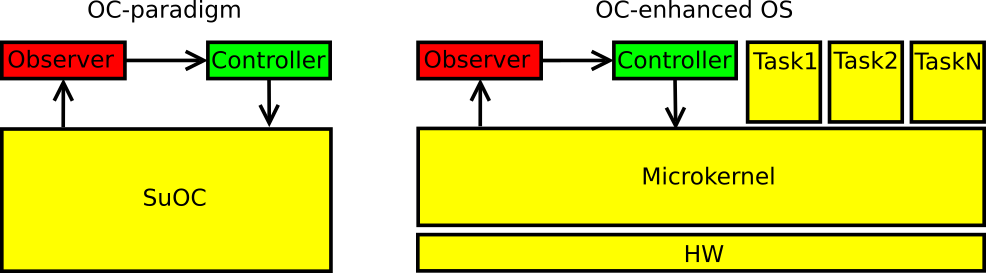
\includegraphics[scale = 0.5]{figures/microkernel_architecture.png}
  \caption{Organic Computing: Applying the Observer/Controller pattern to existing microkernel architecture}\label{architeture}
\end{figure}

\section{Thesis structure}
The thesis is structured in a way that the reader understands the importance of the work carried out here and also the surrounding concepts before delving in to the specifics (inverted traingle). 

The second chapter summarizes the related work on the state of the art algorithms for synchronization and different types of schedulers in use and at the end of the section an evaluation of the synchronization methods is provided inorder to chose the best possible approach for the existing project.

The third chapter explains the Genode and L4 Fiasco.OC details in brief, in order for the user to have an overview of the system. 

The fourth chapter deals with the design considerations along with implementation details.

The fifth chapter is dedicated to explains testing method and the results obtained.
And the final chapter concludes the thesis with the limitations and future work to be done. 
